\documentclass[10pt]{article}

\usepackage[T1]{fontenc}
\usepackage{geometry}
\usepackage{amsmath, amssymb, amsthm}
\usepackage{graphicx}
\usepackage{float}
\usepackage{multirow}
\usepackage{bm}
\usepackage{hyperref}

\geometry{a4paper, margin=1in}

\renewcommand{\labelenumi}{(\alph{enumi})}
\renewcommand{\vec}{\bm}

\newcounter{prob}
\newcommand{\problem}{\stepcounter{prob}\paragraph{Exercise \arabic{prob}}}
\newcommand{\solution}{\paragraph{Solution}}

\newcommand{\C}{\mathbb{C}}
\newcommand{\R}{\mathbb{R}}
\newcommand{\Q}{\mathbb{Q}}
\newcommand{\Z}{\mathbb{Z}}
\newcommand{\N}{\mathbb{N}}

\setlength{\parindent}{0em}

\title{Exercise Sheet I}
\author{Satvik Saha}
\date{}

\begin{document}
    \noindent\textbf{IISER Kolkata} \hfill \textbf{Assignment I}
    \vspace{3pt}
    \hrule
    \vspace{3pt}
    \begin{center}
    \LARGE{\textbf{MA4106: Statistics II}}
    \end{center}
    \vspace{3pt}
    \hrule
    \vspace{3pt}
    Satvik Saha, \texttt{19MS154} \hfill \today
    \vspace{20pt}

    \setlength{\parskip}{1em}


    \section{Introduction}

    Here, we perform linear regression on the Boston house-price dataset;
    specifically, we regress the logarithm of \texttt{MEDV} (the median value of
    owner-occupied homes in units of \$1000) against 13 variables. The values $Y_i$,
    of the dependent variable, where $i$ runs over the $N$ row indices of data
    entries, have been assembled in the column vector $\vec{Y}$. Similarly, the
    values of $X_{ij}$ of the independent variables, where $i$ runs through the row
    indices and $j = 1, \dots, 13$ runs through the variable indices, have been
    assembled in the $N\times 14$ matrix $\vec{X}$. Note that the first column
    $\vec{X}_0$ has been filled with $1$'s. We now use the linear model \[
        \vec{Y} = \vec{X}\beta + \epsilon,
    \] where $\beta$ is a column vector, and $\epsilon$ is a multivariate normal
    random variable with zero mean, covariance matrix $\sigma^2\mathbb{I}_N$.

    \begin{figure}[H]
    \begin{center}
        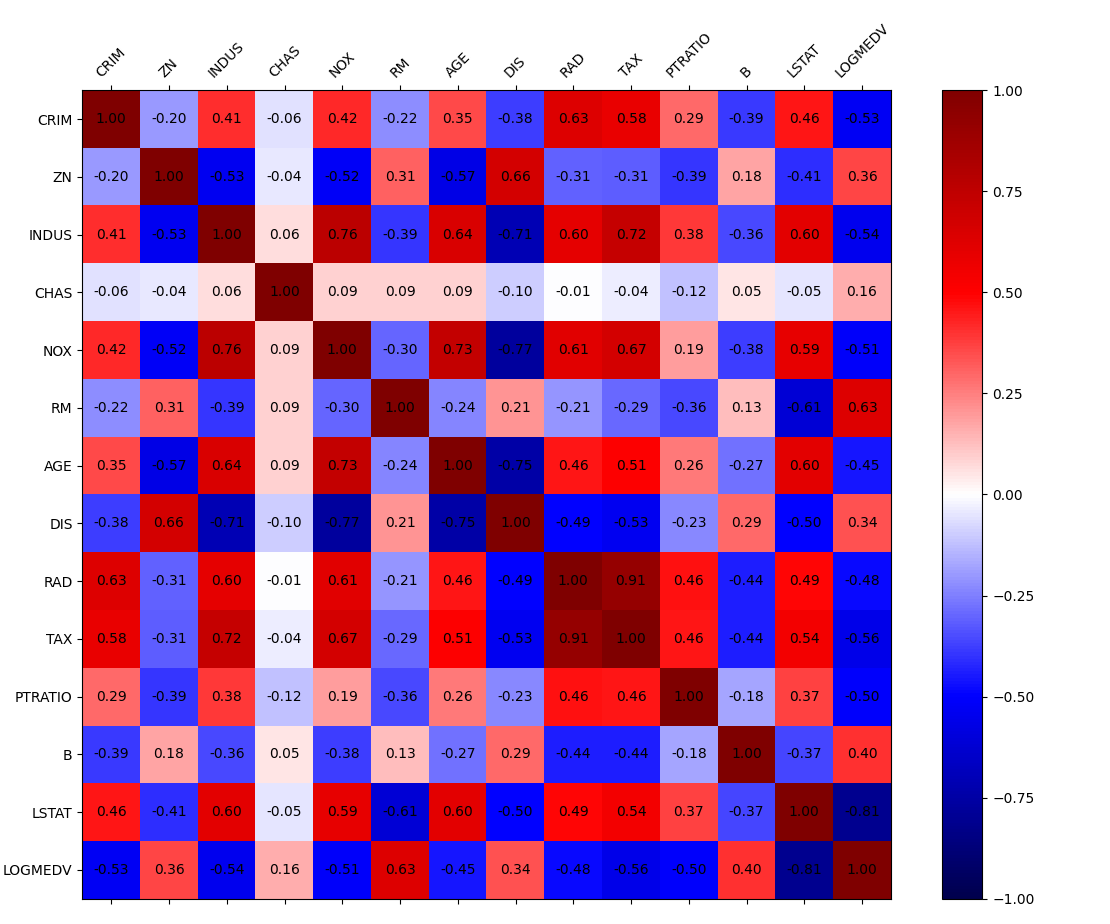
\includegraphics[width=0.9\textwidth]{correlation.png}
    \end{center}
    \caption{
        Correlation matrix between the different variables. Here, \texttt{LOGMEDV}
        denotes the (natural) logarithm of \text{MEDV}. Note the strong positive
        correlation between the variables \texttt{RAD} and \texttt{TAX}. This may
        lead to a problem of multicollinearity.
    }
    \label{fig:correlation}
    \end{figure}

    \begin{table}[H]
    \centering
    \begin{tabular}{|r|r|l|} \hline
        $j$ & Variable          & Description \\\hline
          1 & \texttt{CRIM}     & Per capita crime rate by town \\
          2 & \texttt{ZN}       & Proportion of residential land zoned for lots over 25,000 sq.ft. \\
          3 & \texttt{INDUS}    & Proportion of non-retail business acres per town \\
          4 & \texttt{CHAS}     & Charles River dummy variable (= 1 if tract bounds river; 0 otherwise) \\
          5 & \texttt{NOX}      & Nitric oxides concentration (parts per 10 million) \\
          6 & \texttt{RM}       & Average number of rooms per dwelling \\
          7 & \texttt{AGE}      & Proportion of owner-occupied units built prior to 1940 \\
          8 & \texttt{DIS}      & Weighted distances to five Boston employment centres \\
          9 & \texttt{RAD}      & Index of accessibility to radial highways \\
         10 & \texttt{TAX}      & Full-value property-tax rate per \$10,000 \\
         11 & \texttt{PTRATIO}  & Pupil-teacher ratio by town \\
         12 & \texttt{B}        & $1000(Bk - 0.63)^2$ where Bk is the proportion of blacks by town \\
         13 & \texttt{LSTAT}    & \% lower status of the population \\
            & \texttt{MEDV}     & Median value of owner-occupied homes in \$1000's \\\hline
    \end{tabular}
    \vspace{1em}
    \caption{Variables and their descriptions.}
    \label{tab:variables}
    \end{table}

    Before performing regression, we normalize the independent variable values via
    \[
        \vec{X}_j^* = \frac{\vec{X}_j - \bar{X_j}}{\sqrt{s_{jj}}}, \qquad
        s_{jj} = \sum_{i = 1}^N (\vec{X}_{ij} - \bar{X_j})^2.
    \] These are then assembled as the columns of the matrix $\vec{X}_s^*$. Then, our
    model becomes \[
        \vec{Y} = \vec{X}_s^*\beta^* + \epsilon.
    \] Here, \[
        \beta_0 = \beta_0^* - \sum_{j = 1}^{13}
        \frac{\beta_j^*\bar{X_j}}{\sqrt{s_{jj}}}, \qquad
        \beta_j = \frac{\beta_j^*}{\sqrt{s_{jj}}}.
    \]


    \section{Ordinary Least Squares linear regression}

    Now, the Ordinary Least Squares estimate of $\beta^*$ is given by \[
        \hat{\beta}^* = ({\vec{X}_s^*}^\top\vec{X}_s^*)^{-1}{\vec{X}_s^*}^\top \vec{Y}.
    \] Using this to predict the response given by the same $N$ data entries gives
    the OLS prediction \[
        \hat{\vec{Y}}_{\text{OLS}} = \vec{X}_s^*\beta^* =
        \vec{X}_s^*({\vec{X}_s^*}^\top\vec{X}_s^*)^{-1}{\vec{X}_s^*}^\top \vec{Y}.
    \] The vector of residuals is given by \[
        \vec{E} = \vec{Y} - \hat{\vec{Y}}_{\text{OLS}}.
    \] The goodness of fit $R^2$ is given by \[
        R^2 = 1 - \frac{\Vert \vec{E}\Vert^2}{\Vert \vec{Y} - \bar{Y}\Vert^2}.
    \]

    Following are the results of OLS linear regression to the given dataset. This
    yields an $R^2$ score of $0.79$.

    \begin{table}[H]
    \centering
    \begin{tabular}{|r|l|r|r|r|} \hline
        $j$ & Variable    & $\hat{\beta}_j^*$
                                        & $\hat{\beta}_j$
                                                        &    Variance Inflation Factor
                                                                      \\\hline
        0   &             & 3.034513    &      4.102042 &             \\
        1   & CRIM        &-1.985444    &     -0.010272 &    1.792192 \\
        2   & ZN          & 0.614496    &      0.001172 &    2.298758 \\
        3   & INDUS       & 0.380297    &      0.002467 &    3.991596 \\
        4   & CHAS        & 0.575847    &      0.100888 &    1.073995 \\
        5   & NOX         &-2.026973    &     -0.778399 &    4.393720 \\
        6   & RM          & 1.434196    &      0.090833 &    1.933744 \\
        7   & AGE         & 0.133223    &      0.000211 &    3.100826 \\
        8   & DIS         &-2.322810    &     -0.049087 &    3.955945 \\
        9   & RAD         & 2.791697    &      0.014267 &    7.484496 \\
        10  & TAX         &-2.370043    &     -0.000626 &    9.008554 \\
        11  & PTRATIO     &-1.861951    &     -0.038271 &    1.799084 \\
        12  & B           & 0.848474    &      0.000414 &    1.348521 \\
        13  & LSTAT       &-4.659487    &     -0.029036 &    2.941491 \\\hline
    \end{tabular}
    \vspace{1em}
    \caption{Parameters obtained via OLS linear regression on the Boston dataset.}
    \label{tab:ols_parameters}
    \end{table}

    \begin{figure}[H]
    \begin{center}
        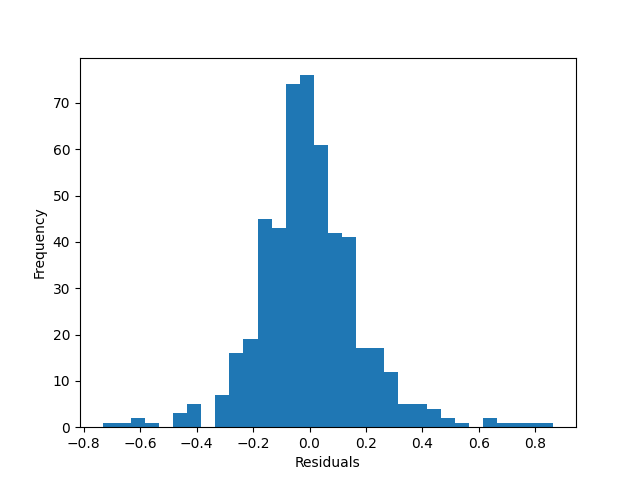
\includegraphics[width=0.8\textwidth]{residuals.png}
    \end{center}
    \caption{Residuals obtained from the OLS linear regression.}
    \label{fig:ols_residuals}
    \end{figure}

    Denoting $\vec{X}^*$ to be the matrix obtained by deleting the first column (of
    1's) from $\vec{X}_s^*$, note that $R_{xx} = {\vec{X}^*}^\top \vec{X}^*$ is
    precisely the correlation matrix of the independent variables. Furthermore, the
    diagonal of $R_{xx}^{-1}$ contains the Variance Inflation Factors of each of the
    variables, calculated in Table~\ref{tab:ols_parameters}. The Variance Inflation
    Factor $\text{VIF}_j$ of the $j$-th variable is so called since \[
        \operatorname{var}(\hat{\beta}_j^*) = \sigma^2 ({\vec{X}^*}^\top
        \vec{X}^*)^{-1}_{jj} = \sigma^2\, \text{VIF}_j.
    \] High VIFs indicate that the estimates $\hat{\beta}_j^*$ for the corresponding
    variables are poor due to their high variance. Note the large VIFs for the
    variables \texttt{RAD} and \texttt{TAX}, which confirms our earlier suspicion
    that they introduce a problem of multicollinearity in our model.


    \section{Ridge regression}

    Here, our estimate of the parameters $\beta^*$ is given by \[
        \hat{\beta}^*(k) = ({\vec{X}_s^*}^\top\vec{X}_s^* +
        k\mathbb{I}_{14})^{-1}{\vec{X}_s^*}^\top \vec{Y}.
    \] This is done to mitigate the problem of multicollinearity, which may cause the
    matrix ${\vec{X}_s^*}^\top \vec{X}_s^*$ to be close to singular.

    Let $\{\lambda_i\}$ be the eigenvalues of the matrix $R_{xx}$. Then, the value
    \[
        \kappa = \sqrt{\frac{\lambda_{max}}{\lambda_{min}}}
    \] is a measure of multicollinearity in the model. In our case, $\kappa \approx
    9.82$.



    \subsection{Ridge-trace plot}


    \begin{figure}[H]
    \begin{center}
        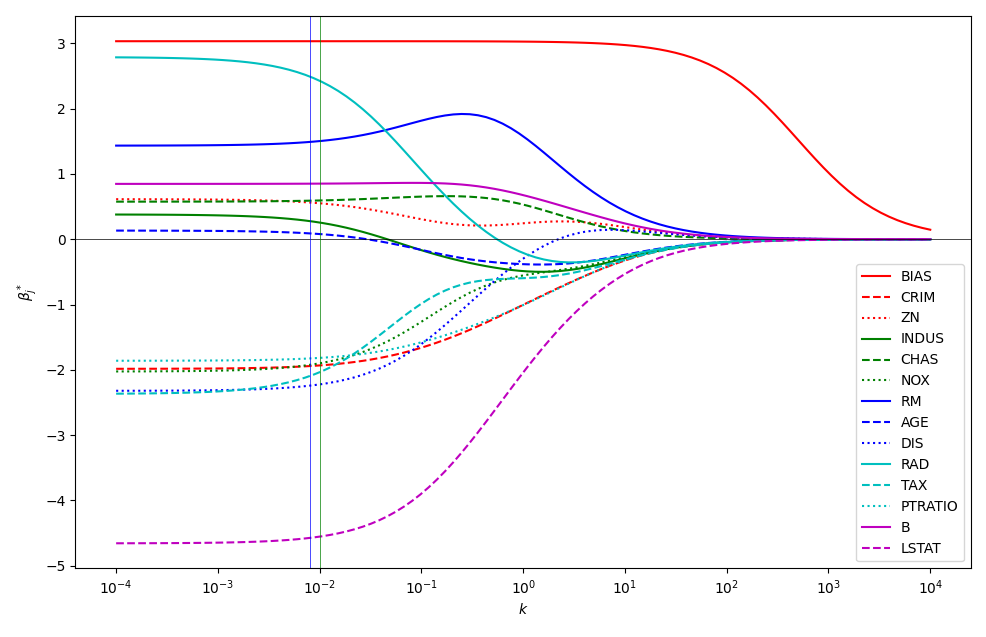
\includegraphics[width=\textwidth]{ridgetrace.png}
    \end{center}
    \caption{
        A ridge-trace plot, showing the variation of the parameters $\beta_j^*$ with
        $k$. It can be seen that each $\beta_j^* \to 0$ as $k \to \infty$. The
        vertical green line marks $k = 0.01$, and the vertical blue line marks $k =
        0.008$. Note that \texttt{BIAS} denotes the `variable' corresponding to the
        parameter $\beta_0$.
    }
    \label{fig:ridge_trace}
    \end{figure}

    The ridge trace plot shows that with increasing $k$, the parameters $\beta_j^*$
    shift from their OLS values and briefly plateau at another value, before decaying
    to zero. This effect is clearest in the curves of \texttt{TAX} and \texttt{ZN},
    both around $k = 1$. Some parameters, like the curves for \texttt{INDUS},
    \texttt{AGE}, \texttt{RAD}, \texttt{DIS}, even change sign. Note that the curves
    for \texttt{RAD} and \texttt{TAX} are the fastest shrinking ones with $k$.

    By a crude visual estimate, we choose $k = 0.01$. This the point (to the nearest
    power of 10) where the some of the OLS estimates begin decaying towards zero.

    Note that the OLS estimates of the parameters (Table~\ref{tab:ols_parameters})
    corresponding to \texttt{INDUS}, \texttt{AGE}, \texttt{RAD} are positive although
    they are negatively correlated with \texttt{LOGMEDV} as per
    Figure~\ref{fig:correlation}. In particular, the parameter corresponding to
    \texttt{RAD} has the third highest magnitude and is positive, despite the
    correlation between \texttt{RAD} and \texttt{LOGMEDV} being $-0.48$. Similarly,
    the OLS estimate of the parameter corresponding to \texttt{DIS} has the fifth
    highest magnitude and is negative, despite the correlation between \texttt{DIS}
    and \texttt{LOGMEDV} being $+0.34$.


    \subsection{Cross validation}

    Another method of choosing a value of $k$ is by minimizing the prediction error
    with respect to $k$. The Prediction Error (PE) has to be estimated via some
    means; here, we use Leave-One-Out Cross Validation (LOOCV). In this process, a
    row $i$ of the dataset is set aside, and the model parameters are determined
    using the remaining rows. These are used to generate a prediction $\hat{Y}_i$ for
    $Y_i$, using the variables in row $i$. This predicted value is compared against
    the true value of row $i$, yielding a prediction error. The above process is
    repeated for each row $i$. Here, we use the mean of squares of prediction errors,
    \[
        \text{PE} \approx \text{LOOCV} = \frac{1}{N}\sum_{i = 1}^N (Y_i - \hat{Y}_i)^2.
    \]

    \begin{figure}[H]
    \begin{center}
        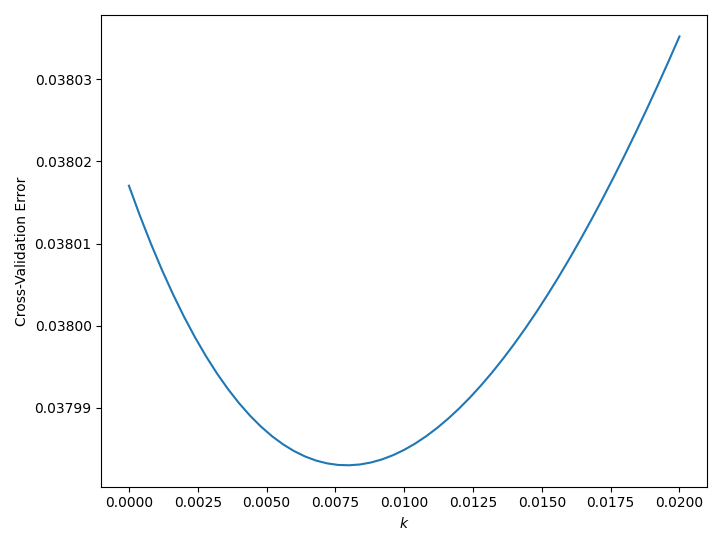
\includegraphics[width=0.8\textwidth]{loocvmse.png}
    \end{center}
    \vspace{-1em}
    \caption{
        The variation of the LOOCV with $k$, which gives an estimate of the
        prediction error.
    }
    \label{fig:loocv}
    \end{figure}

    In our case, the LOOCV is minimized at $k = 0.008$. The LOOCV surpasses its OLS
    ($k = 0$) value beyond $k = 0.017$.


    \section{Conclusion}


    \begin{table}[H]
    \centering
    \begin{tabular}{|r|l|r|r|r|r|r|r|} \hline
        \multirow{2}{*}{$j$}
            & \multirow{2}{*}{Variable}
                          & \multicolumn{3}{c|}{$\hat{\beta}^*_j(k)$}
                                                                      &
                                                                      \multicolumn{3}{c|}{$\hat{\beta}_j(k)$}
                                                                                                          \\\cline{3-8}
            &             & \multicolumn{1}{c|}{$k = 0$}
                                          & \multicolumn{1}{c|}{$k = 0.008$}
                                                          & \multicolumn{1}{c|}{$k = 0.010$}
                                                                      & \multicolumn{1}{c|}{$k = 0$}
                                                                                   & \multicolumn{1}{c|}{$k = 0.008$}
                                                                                               & \multicolumn{1}{c|}{$k = 0.010$}
                                                                                                          \\\hline
        0   &             & 3.034513      &  3.034465     & 3.034453  & 4.102042   & 4.028287  & 4.010485 \\
        1   & CRIM        &-1.985444      & -1.943415     &-1.933262  &-0.010272   &-0.010054  &-0.010002 \\
        2   & ZN          & 0.614496      &  0.563474     & 0.551583  & 0.001172   & 0.001075  & 0.001052 \\
        3   & INDUS       & 0.380297      &  0.278933     & 0.255974  & 0.002467   & 0.001809  & 0.001660 \\
        4   & CHAS        & 0.575847      &  0.590940     & 0.594359  & 0.100888   & 0.103532  & 0.104131 \\
        5   & NOX         &-2.026973      & -1.925292     &-1.900518  &-0.778399   &-0.739352  &-0.729838 \\
        6   & RM          & 1.434196      &  1.490724     & 1.504286  & 0.090833   & 0.094413  & 0.095272 \\
        7   & AGE         & 0.133223      &  0.090123     & 0.079812  & 0.000211   & 0.000142  & 0.000126 \\
        8   & DIS         &-2.322810      & -2.243870     &-2.223905  &-0.049087   &-0.047419  &-0.046997 \\
        9   & RAD         & 2.791697      &  2.495783     & 2.427773  & 0.014267   & 0.012755  & 0.012407 \\
        10  & TAX         &-2.370043      & -2.098250     &-2.037197  &-0.000626   &-0.000554  &-0.000538 \\
        11  & PTRATIO     &-1.861951      & -1.826501     &-1.817834  &-0.038271   &-0.037543  &-0.037365 \\
        12  & B           & 0.848474      &  0.851608     & 0.852371  & 0.000414   & 0.000415  & 0.000415 \\
        13  & LSTAT       &-4.659487      & -4.577014     &-4.556287  &-0.029036   &-0.028522  &-0.028392 \\\hline
    \end{tabular}
    \vspace{1em}
    \caption{Parameter estimates for selected values of $k$.}
    \label{tab:all_parameters}
    \end{table}

    The $R^2$ values corresponding to the ridge regressions with $k = 0, 0.008, 0.010$
    have been calculated as $0.7896, 0.7894, 0.793$ respectively.
    Figure~\ref{fig:loocv} shows that the estimated prediction error for $k =
    0.010$ is slightly greater than that for $k = 0.008$. Thus, we choose the ridge
    regression parameter $0.008$, as it minimizes the estimated prediction error.
    This choice does not contradict the ridge-trace plot either.

    Also note that we have calculated $\kappa < 10$, which does not seem to indicate
    much of a problem with multicollinearity. The main variables under suspicion here
    are \texttt{RAD} and \texttt{TAX} which are highly correlated; simply removing
    one of the two may yield a better performing model than one obtained via ridge
    regression. Removing some of the variables which change sign in the ridge-trace
    plot (Figure~\ref{fig:ridge_trace}) may also yield some improvement.

    With this in mind, we also prefer the ridge estimates to the OLS ones; the ridge
    estimates give better (estimated) prediction errors, with lower variance
    inflations.


\end{document}
